\documentclass{beamer}
\colorlet{structure}{green!50!black}

\mode<article> % only for the article version
{
  \usepackage{fullpage}
  \usepackage{hyperref}
}
\mode<presentation>
{
	\setbeamertemplate{background canvas}[vertical shading][bottom=red!10,top=blue!10]
%	\useinnertheme[shadow=true]{rounded}
%	\useoutertheme{shadow}
%	\usecolortheme{whale}
	\setbeamerfont{block title}{size={}}
  \usefonttheme[onlysmall]{structurebold}
}

\setbeamersize{mini frame size=5cm}

\usepackage[english]{varioref}

\usetheme{Hannover}
\usecolortheme{dove}
%\setbeamercolor{math text}{fg=green!50!black}
%\setbeamercolor{normal text in math text}{parent=math text}

%\usepackage{pgf,pgfarrows,pgfnodes,pgfautomata,pgfheaps,pgfshade}
\usepackage{amsmath,amssymb}
%\usepackage[latin1]{inputenc}
\usepackage[utf8]{inputenc}
\usepackage{colortbl}
\usepackage[english,german,ngerman]{babel}
% Line spacing
\usepackage{setspace}
\usepackage{listings}
%\usepackage{lmodern}
%\usepackage[T1]{fontenc}
\usepackage{times}
\setbeamercovered{dynamic}

%
% The following defintions are peculiar to this particular
% presetation. They have nothing to do with the beamer class
%

\newcommand{\Lang}[1]{\operatorname{\text{\textsc{#1}}}}

\newcommand{\Class}[1]{\operatorname{\mathchoice
  {\text{\normalfont\small #1}}
  {\text{\normalfont\small #1}}
  {\text{\normalfont#1}}
  {\text{\normalfont#1}}}}

\newcommand{\DOF}{\Class{DOF}}
\newcommand{\NOF}{\Class{NOF}}
\newcommand{\DOFpoly}{\Class{DOF}_{\operatorname{poly}}}
\newcommand{\NOFpoly}{\Class{NOF}_{\operatorname{poly}}}

\newcommand{\Nat}{\mathbb{N}}
\newcommand{\Set}[1]{\{#1\}}

\newenvironment{ccodelisting}
{\begin{list}{}{\setlength{\leftmargin}{1em}}\item\scriptsize\bfseries}
{\end{list}}


%
% The following info should normally be given in you main file:
%
%\subject{cryptographic primitives}
%\lstset{
%	language=ADA,
%        basicstyle=\ttfamily,
%        keywordstyle=\color{Red},
%        commentstyle=\color{Blue},
%        stringstyle=\color{Green},
%        showstringspaces=false,
%        emph={bool,int,unsigned,char,true,false,void}, %emphstyle=\color{CornflowerBlue},
%        emph={[2]IFF\_TUN}, emphstyle={[2]\color{red}}
%}

\author{S\"oren Heisrath \and Daniel Otte}
\title{AnonAccess}
\institute{
\includegraphics[scale=0.25]{laborlogo.png}}
\date[21. Dezember 2007]{21.12.2007}

\begin{document}

%-------------------------------------------------------------------------------

\frame{\titlepage}

\section<presentation>*{}

\begin{frame}
  \frametitle{}
  \tableofcontents[part=1,pausesection,hideallsubsections]
\end{frame}

%\AtBeginSubsection[]
%\AtBeginSection[]
%{
%  \begin{frame}<beamer>
%    \frametitle{"Ubersicht}
%    \tableofcontents[currentsection]
%    %\tableofcontents[current,currentsubsection]
%  \end{frame}
%}

\part<presentation>{Intro}
\section{Anforderungen \& Beispiele}
\begin{frame}
	\frametitle{Anforderungen}
	\begin{itemize}
		\item<2-> Wartbarkeit
		\item<3-> Kryptografische Sicherheit
		\item<4-> Physikalische Sicherheit
		\item<5-> Kleines \& Energieeffizientes System
		\item<6-> Anonymit"at
	\end{itemize}
\end{frame}
\begin{frame}
	\frametitle{Wartbarkeit}
	\begin{itemize}
		\item<2-> Hinzuf"ugen von Nutzern
		\item<3-> L"oschen von Nutzern
		\item<4-> Privilegien verwalten
	\end{itemize}
\end{frame}
\begin{frame}
	\frametitle{Kryptografische Sicherheit}
	\begin{itemize}
		\item<2-> Sicherung des Kanals
		\item<3-> Sichere Speicherung der Datenbank
		\item<4-> Kryptografisch sicherer Zufallsgenerator
	\end{itemize}
\end{frame}

\begin{frame}
	\frametitle{Physikalische Sicherheit}
	\begin{itemize}
		\item<2-> Sicherung gegen "offnen des Geh"auses
		\item<3-> Sichere L"oschung der Daten
	\end{itemize}
\end{frame}

\begin{frame}
	\frametitle{Hardwareanforderungen}
	\begin{itemize}
		\item<2-> Microcontroller Plattform
		\item<3-> USV Sicherung f"ur mehrere Tage
	\end{itemize}
\end{frame}

\section{Aufbau}
\begin{frame}
\frametitle{Grundaufbau}
	\begin{center}
		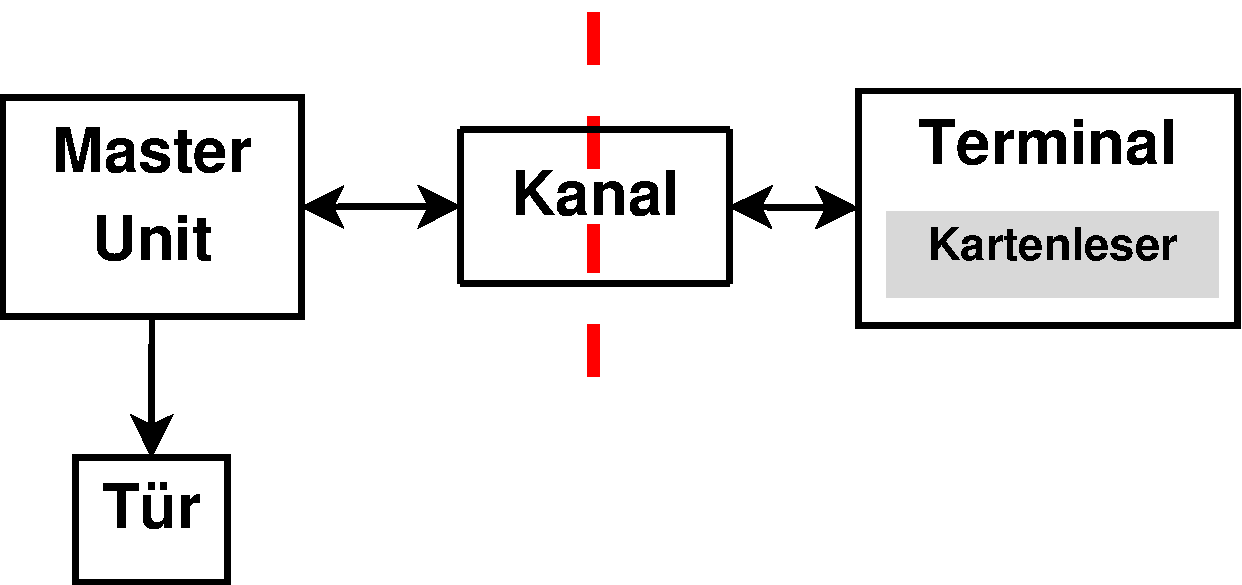
\includegraphics[width=210px]{grundaufbau}
	\end{center}
\end{frame}

\begin{frame}
\frametitle{Master Unit}
	\begin{itemize}
		\item<2-> Speicherung der Datenbank
		\item<3-> Authentifizierung der Nutzer
		\item<4-> L"oschung der Schl"ussel \& Datenbank bei physikalischen Angriffen
		\item<5-> USV
	\end{itemize}
\end{frame}

\begin{frame}
\frametitle{Panel}
	\begin{itemize}
		\item<2-> Weitergabe der Kartendaten
		\item<3-> Ein- und Ausgabe \small{(Master Unit <-> Mensch)}
		\item<4-> L"oschung des Schl"ussels bei physikalischen Angriffen
	\end{itemize}
\end{frame}

\begin{frame}
\frametitle{Kanal}
	Galvanische Trennung zwischen Master Unit und Panel
\end{frame}

\section{M"ogliche (alternative) Implementationen}
\begin{frame}
	\frametitle{Variante 1}
	\textbf{''}Speicherung von Einmal-Tokens zusammen\\
	mit ID oder Nickname in einer\\
	Datenbank \& auf der Karte\textbf{''}

	\vspace{1cm}\par

	\textbf<2->{Nachteil:}
	\begin{itemize}
		\item<2-> Pseudonyme sind nicht ganz so anonym
	\end{itemize}
\end{frame}

\begin{frame}
	\frametitle{Variante 2}
	\textbf{''}Generieren von neuen IDs\\
	und Tokens bei jedem login\textbf{''}

	\vspace{1cm}

	\textbf<2->{Nachteil:}
	\begin{itemize}
		\item<2-> Nicht wartbar
	\end{itemize}
\end{frame}

\begin{frame}
	\frametitle {Neue Problemstellungen}
	\begin{itemize}
		\item<2-> Speicherung von lesbaren Informationen auf der
		Karte ist eine schlechte Idee.
		\item<3-> Die Nutzerdatenbank sollte gesch"utzt werden.
	\end{itemize}
\end{frame}

\begin{frame}
	\frametitle{Das Problem der Wartbarkeit}
	Zwei Alternativen:
	\begin{enumerate}
		\item<2-> Nutzer Pseudonyme
		\item<3-> Timeouts
	\end{enumerate}
\end{frame}

\section{AnonAccess Konzept}

\begin{frame}
	\frametitle {Neue Problemstellungen}
	Das Problem der Wartbarkeit
	\begin{itemize}
		\item<2-> Nutzer müssen adressierbar sein.
		\item<3-> Lösungsidee: Nutzer müssen nicht die ganze Zeit adressierbar sein.
	\end{itemize}
\end{frame}

\begin{frame}
	\frametitle {Lösung}
	Änderungen an einem Benutzerkonto werden erst dann angewendet wenn sich der Benutzer anmeldet.
	Die Adressierung findet über einen sogenannten Nickname statt.\\
	Dieser Nickname wird jedoch nirgwendwo im Klartext gespeichert.\\
	Auf der Karte wird ein verschlüsselter Fingerprint des Nicknames gespeichert.\\
\end{frame}

\begin{frame}
	\frametitle {Lösung}
	Sollen die Eigenschaften eines Kontos modifiziert werden,\\
	dann wird ein Eintrag in der Flag-Modify-Database erstellt.
	\begin{itemize}
	\item<2-> Fingerprint des Nicknames
	\item<3-> Änderungsanweisungen
	\end{itemize}
\end{frame}

\begin{frame}
	\frametitle {Lösung}
	Nun wird der Ablauf der Authentifizierung erweitert um:
	\begin{itemize}
	\item<2-> Entschlüsseln des Nickname Fingerprints
	\item<3-> Suche in der Datenbank nach Änderungen für dieses Konto
	\end{itemize}
\end{frame}


\section{Implementationen}
\begin{frame}
	\frametitle{Begriffe}
	\begin{large}Token\end{large}
	\\
	Einmal verwendbarer Datensatz zur Authentifikation

	\vspace{1cm}

	\begin{large}Flags\end{large}
	\\
	Meta Informationen "uber den Zustand eines Nutzers.
	\begin{itemize}
		\item \texttt{active}: Benutzeraccount aktiv
		\item \texttt{permanent}: Benutzeraccount darf beliebig oft verwendet werden
		\item \texttt{hnick}: HMAC des Pseudonyms
	\end{itemize}
\end{frame}

\begin{frame}
	\frametitle{Speicherung von Tokens}
	\begin{itemize}
		\item<2-> Cipher: Shabea-16
		\item<3-> EEPROM geteilt in 32 Byte Bl"ocke
		\item<4-> 32-Byte Bl"ocke jew. mit eigenem Schl"ussel
	\end{itemize}
\end{frame}


\begin{frame}
	\frametitle{Speicherung von Tickets}
	Was wird gespeichert?
	\begin{itemize}
		\item<2-> HMAC des Tokens
		\item<3-> ID des Users
		\item<4-> Versionsnummer
		\item<5-> Nutzerrechte/Flags
	\end{itemize}
\end{frame}

\begin{frame}
	\frametitle{Schl"usselhierarchie}
	TBD.
\end{frame}


% ----

\end{document}

